% -*- LaTeX -*-
% -*- coding: utf-8 -*-
%
% ~~~~~~~~~~~~~~~~~~~~~~~~~~~~~~~~~~~~~~~~~~~~~~~~~~~~~~~~~~~~~~~~~~~~~~~~~~~~~~
%
%                             michael a.g. aïvázis
%                      california institute of technology
%                      (c) 1998-2010  all rights reserved
%
% ~~~~~~~~~~~~~~~~~~~~~~~~~~~~~~~~~~~~~~~~~~~~~~~~~~~~~~~~~~~~~~~~~~~~~~~~~~~~~~
%

\lecture{Programming NVidia GPUs with CUDA}{20100129}

% --------------------------------------
% template
\begin{frame}[fragile]
%
  \frametitle{Hybrid architectures}
%
  \begin{itemize}
%
  \item recall the layout of SIMD machines
    \begin{itemize}
    \item a large number of small, special purpose processors
    \item a single ``controller'' manages the instruction stream
      \begin{itemize}
      \item each processor executes the same instruction on its local data
      \item may be able to specify which processors are active/idle
      \end{itemize}
    \end{itemize}
    \begin{figure}
      \centering
      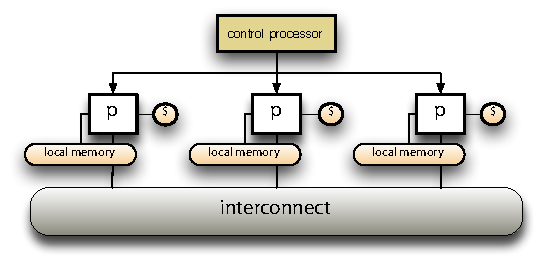
\includegraphics[width=.50\linewidth]{figures/simd.pdf}
      \label{fig:simd}
    \end{figure}
%
  \item modern hybrid systems based on GPUs have somewhat more elaborate architectures
    \begin{itemize}
      \item multi-tier memory layouts
      \item large core counts per board
      \item elaborate access rules that enable the hardware to be very fast
      \item recent ones finally support double precision floating point arithmetic
      \item broadly available -- it's in your graphics card, thanks to video gaming
    \end{itemize}
%
  \end{itemize}
%
\end{frame}

% --------------------------------------
% CUDA architecture
\begin{frame}[fragile]
%
  \frametitle{nVidia GPU architecture}
%
  \begin{itemize}
  \item The GPU boards are hosted by a conventional processor
    \begin{itemize}
    \item connected through PCI Express, which is the limiting factor in moving data to and
      from the device memory
    \end{itemize}
  \item computing power and memory configurations vary from
    \begin{itemize}
    \item a single 2-core GPU with 128M of memory on older video cards
    \item to 30 $\times$ 8-core SIMTs with 4G of memory on the Tesla C1060
      \begin{itemize}
      \item 240 cores; peak: 933 Gflops single precision, 78 Gflops double precision
      \item rivulet.cacr.caltech.edu has four such boards
      \end{itemize}
    \end{itemize}
  \end{itemize}  
  
%
  \begin{figure}
    \centering
    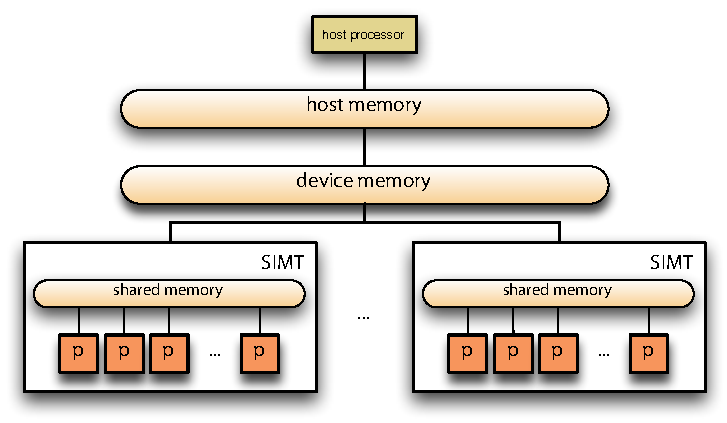
\includegraphics[width=0.75\linewidth]{figures/cuda-architecture.pdf}
    \label{fig:simd}
  \end{figure}
%
\end{frame}

% --------------------------------------
% getting started
\begin{frame}[fragile]
%
  \frametitle{Getting started}
%
  \begin{itemize}
%
  \item getting the drivers, tools and code samples
    \begin{itemize}
    \item visit \href{http://nvidia.com/cuda}
    \end{itemize}
%
  \item compiling and linking
    \begin{itemize}
    \item \cc\ for CUDA: a few extensions
    \item source is a mixture of the code that runs on the host and the {\em kernels} that run
      on the \identifier{GPU}
    \item there are restrictions on what kind of code you can include in a kernel
    \item \identifier{nvcc} is the special compiler and linker
    \end{itemize}
%
  \item staging and launching
    \begin{itemize}
    \item the resulting executable runs on the hosts
    \item launches threads on the GPU through special statements
    \end{itemize}
%
  \item the emulator
    \begin{itemize}
    \item the SDK comes with a software emulator
    \item extremely useful for debugging
    \end{itemize}
%
  \item special hardware
    \begin{itemize}
    \item your video card
    \item Tesla boards
    \end{itemize}
%
  \end{itemize}
%
\end{frame}

% --------------------------------------
% sanity check
\begin{frame}[fragile]
%
  \frametitle{Sanity check}
  \label{slide:sanity-cuda}
%
  \begin{C}[basicstyle=\tt\bfseries\tiny]
#include <cuda.h>
#include <assert.h>

int main(int argc, char* argv[]) {
    int i;
    int N = 12;
    // allocate some buffers on the host
    float *send_host = (float *) malloc(N*sizeof(float));
    float *recv_host = (float *) malloc(N*sizeof(float));
    // allocate matching ones on the device
    float *send_device, *recv_device;
    cudaMalloc((void **) &recv_device, N*sizeof(float));
    cudaMalloc((void **) &send_device, N*sizeof(float));
    // and initialize the host data
    for (i=0; i<N; i++) {
        send_host[i] = 2.0f + i*i;
        recv_host[i] = 0.0f;
    }
    // send the data from the host to the device
    cudaMemcpy(recv_device, send_host, N*sizeof(float), cudaMemcpyHostToDevice);
    // move the data in device memory
    cudaMemcpy(send_device, recv_device, N*sizeof(float), cudaMemcpyDeviceToDevice);
    // get it back on the host
    cudaMemcpy(recv_host, send_device, N*sizeof(float), cudaMemcpyDeviceToHost);
    // check the result
    for (i=0; i<N; i++) {
      assert(send_host[i] == recv_host[i]);
    }
    // free the buffers;
    free(send_host)l free(recv_host);
    cudaFree(send_device); cudaFree(recv_device);

    return 0;
}
  \end{C}
%
\end{frame}

% --------------------------------------
% programming model
\begin{frame}[fragile]
%
  \frametitle{The programming model fundamentals}
%
  \begin{itemize}
%
  \item memory
%
  \item thread granularity
%
  \end{itemize}
%
\end{frame}

% --------------------------------------
% the execution model
\begin{frame}[fragile]
%
  \frametitle{The execution model}
%
  \begin{itemize}
%
  \item 
%
  \end{itemize}
%
\end{frame}

% --------------------------------------
% hello world
\begin{frame}[fragile]
%
  \frametitle{Hello world -- not!}
  \label{slide:hello-world-cuda}
%
  \begin{C}
// kernel
__global__ void vec_add(double* a, double* b, double* c) {
    int i = threadIdx.x;
    c[i] = a[i] + b[a];
}

int main(int argc, char* argv[]) {
  // invoke the kernel
  vec_add <<<1,N>>> (a,b,c);

  return 0;
}
  \end{C}
%
\end{frame}

% end of file 
